\documentclass[11pt,twoside,letterpaper]{article}
\newcommand{\reporttitle}{Lab 3: Localization with an Extended Kalman Filter}
\newcommand{\reportauthorOne}{Adams, Hunter}
\newcommand{\cidOne}{20997503}
\newcommand{\reportauthorTwo}{Chen, Joe}
\newcommand{\cidTwo}{20998545}
\newcommand{\reportauthorThree}{Wielowieyski, Jacob}
\newcommand{\cidThree}{21004619}
% ---- FILL IN: station and robot number used in the Lab 3 session ----
\newcommand{\robotNumber}{7}
\newcommand{\stationNumber}{\textcolor{red}{FILL IN}}
\date{\today}
%%%%%%%%%%%%%%%%%%%%%%%%%%%%%%%%%%%%%%%%%
% University Assignment Title Page 
% LaTeX Template
% Version 1.0 (27/12/12)
%
% This template has been downloaded from:
% http://www.LaTeXTemplates.com
%
% Original author:
% WikiBooks (http://en.wikibooks.org/wiki/LaTeX/Title_Creation)
%
% License:
% CC BY-NC-SA 3.0 (http://creativecommons.org/licenses/by-nc-sa/3.0/)
% 
% Instructions for using this template:
% This title page is capable of being compiled as is. This is not useful for 
% including it in another document. To do this, you have two options: 
%
% 1) Copy/paste everything between \begin{document} and \end{document} 
% starting at \begin{titlepage} and paste this into another LaTeX file where you 
% want your title page.
% OR
% 2) Remove everything outside the \begin{titlepage} and \end{titlepage} and 
% move this file to the same directory as the LaTeX file you wish to add it to. 
% Then add \input{./title_page_1.tex} to your LaTeX file where you want your
% title page.
%
%----------------------------------------------------------------------------------------
%	PACKAGES AND OTHER DOCUMENT CONFIGURATIONS
%----------------------------------------------------------------------------------------
\usepackage{ifxetex}
\usepackage{textpos}
\usepackage{natbib}
\usepackage{kpfonts}
\usepackage[letterpaper,hmargin=2.8cm,vmargin=2.0cm,includeheadfoot]{geometry}
\usepackage{ifxetex}
\usepackage{stackengine}
\usepackage{tabularx,longtable,multirow,subfigure,caption}%hangcaption
\usepackage{fncylab} %formatting of labels
\usepackage{fancyhdr}
\usepackage{color}
\usepackage[tight,ugly]{units}
\usepackage{url}
\usepackage{float}
\usepackage[english]{babel}
\usepackage{amsmath}
\usepackage{graphicx}
\usepackage[colorinlistoftodos]{todonotes}
\usepackage{dsfont}
\usepackage{epstopdf} % automatically replace .eps with .pdf in graphics
\usepackage{natbib}
\usepackage{backref}
\usepackage{array}
\usepackage{latexsym}
\usepackage{etoolbox}

\usepackage{enumerate} % for numbering with [a)] format 



\ifxetex
\usepackage{fontspec}
\setmainfont[Scale=.8]{OpenDyslexic-Regular}
\else
\usepackage[pdftex,pagebackref,hypertexnames=false,colorlinks]{hyperref} % provide links in pdf
\hypersetup{pdftitle={},
  pdfsubject={}, 
  pdfauthor={\reportauthorOne},
  pdfkeywords={}, 
  pdfstartview=FitH,
  pdfpagemode={UseOutlines},% None, FullScreen, UseOutlines
  bookmarksnumbered=true, bookmarksopen=true, colorlinks,
    citecolor=black,%
    filecolor=black,%
    linkcolor=black,%
    urlcolor=black}
\usepackage[all]{hypcap}
\fi

\usepackage{tcolorbox}

% various theorems
\usepackage{ntheorem}
\theoremstyle{break}
\newtheorem{lemma}{Lemma}
\newtheorem{theorem}{Theorem}
\newtheorem{remark}{Remark}
\newtheorem{definition}{Definition}
\newtheorem{proof}{Proof}

% example-environment
\newenvironment{example}[1][]
{ 
\vspace{4mm}
\noindent\makebox[\linewidth]{\rule{\hsize}{1.5pt}}
\textbf{Example #1}\\
}
{ 
\noindent\newline\makebox[\linewidth]{\rule{\hsize}{1.0pt}}
}



%\renewcommand{\rmdefault}{pplx} % Palatino
% \renewcommand{\rmdefault}{put} % Utopia

\ifxetex
\else
\renewcommand*{\rmdefault}{bch} % Charter
\renewcommand*{\ttdefault}{cmtt} % Computer Modern Typewriter
%\renewcommand*{\rmdefault}{phv} % Helvetica
%\renewcommand*{\rmdefault}{iwona} % Avant Garde
\fi

\setlength{\parindent}{0em}  % indentation of paragraph

\setlength{\headheight}{14.5pt}
\pagestyle{fancy}
\fancyfoot[ER,OL]{\thepage}%Page no. in the left on
                                %odd pages and on right on even pages
\fancyfoot[OC,EC]{\sffamily }
\renewcommand{\headrulewidth}{0.1pt}
\renewcommand{\footrulewidth}{0.1pt}
\captionsetup{margin=10pt,font=small,labelfont=bf}


%--- chapter heading

\def\@makechapterhead#1{%
  \vspace*{10\p@}%
  {\parindent \z@ \raggedright %\sffamily
        %{\Large \MakeUppercase{\@chapapp} \space \thechapter}
        %\\
        %\hrulefill
        %\par\nobreak
        %\vskip 10\p@
    \interlinepenalty\@M
    \Huge \bfseries 
    \thechapter \space\space #1\par\nobreak
    \vskip 30\p@
  }}

%---chapter heading for \chapter*  
\def\@makeschapterhead#1{%
  \vspace*{10\p@}%
  {\parindent \z@ \raggedright
    \sffamily
    \interlinepenalty\@M
    \Huge \bfseries  
    #1\par\nobreak
    \vskip 30\p@
  }}
  



% %%%%%%%%%%%%% boxit
\def\Beginboxit
   {\par
    \vbox\bgroup
	   \hrule
	   \hbox\bgroup
		  \vrule \kern1.2pt %
		  \vbox\bgroup\kern1.2pt
   }

\def\Endboxit{%
			      \kern1.2pt
		       \egroup
		  \kern1.2pt\vrule
		\egroup
	   \hrule
	 \egroup
   }	

\newenvironment{boxit}{\Beginboxit}{\Endboxit}
\newenvironment{boxit*}{\Beginboxit\hbox to\hsize{}}{\Endboxit}



\allowdisplaybreaks

\makeatletter
\newcounter{elimination@steps}
\newcolumntype{R}[1]{>{\raggedleft\arraybackslash$}p{#1}<{$}}
\def\elimination@num@rights{}
\def\elimination@num@variables{}
\def\elimination@col@width{}
\newenvironment{elimination}[4][0]
{
    \setcounter{elimination@steps}{0}
    \def\elimination@num@rights{#1}
    \def\elimination@num@variables{#2}
    \def\elimination@col@width{#3}
    \renewcommand{\arraystretch}{#4}
    \start@align\@ne\st@rredtrue\m@ne
}
{
    \endalign
    \ignorespacesafterend
}
\newcommand{\eliminationstep}[2]
{
    \ifnum\value{elimination@steps}>0\leadsto\quad\fi
    \left[
        \ifnum\elimination@num@rights>0
            \begin{array}
            {@{}*{\elimination@num@variables}{R{\elimination@col@width}}
            |@{}*{\elimination@num@rights}{R{\elimination@col@width}}}
        \else
            \begin{array}
            {@{}*{\elimination@num@variables}{R{\elimination@col@width}}}
        \fi
            #1
        \end{array}
    \right]
    & 
    \begin{array}{l}
        #2
    \end{array}
    &%                                    moved second & here
    \addtocounter{elimination@steps}{1}
}
\makeatother

%% Fast macro for column vectors
\makeatletter  
\def\colvec#1{\expandafter\colvec@i#1,,,,,,,,,\@nil}
\def\colvec@i#1,#2,#3,#4,#5,#6,#7,#8,#9\@nil{% 
  \ifx$#2$ \begin{bmatrix}#1\end{bmatrix} \else
    \ifx$#3$ \begin{bmatrix}#1\\#2\end{bmatrix} \else
      \ifx$#4$ \begin{bmatrix}#1\\#2\\#3\end{bmatrix}\else
        \ifx$#5$ \begin{bmatrix}#1\\#2\\#3\\#4\end{bmatrix}\else
          \ifx$#6$ \begin{bmatrix}#1\\#2\\#3\\#4\\#5\end{bmatrix}\else
            \ifx$#7$ \begin{bmatrix}#1\\#2\\#3\\#4\\#5\\#6\end{bmatrix}\else
              \ifx$#8$ \begin{bmatrix}#1\\#2\\#3\\#4\\#5\\#6\\#7\end{bmatrix}\else
                 \PackageError{Column Vector}{The vector you tried to write is too big, use bmatrix instead}{Try using the bmatrix environment}
              \fi
            \fi
          \fi
        \fi
      \fi
    \fi
  \fi 
}  
\makeatother

\robustify{\colvec}

%%% Local Variables: 
%%% mode: latex
%%% TeX-master: "notes"
%%% End: 

% quick way of adding a figure
\newcommand{\fig}[3]{
 \begin{center}
 \scalebox{#3}{\includegraphics[#2]{#1}}
 \end{center}
}

%\newcommand*{\point}[1]{\vec{\mkern0mu#1}}
\newcommand{\ci}[0]{\perp\!\!\!\!\!\perp} % conditional independence
\newcommand{\point}[1]{{#1}} % points 
\renewcommand{\vec}[1]{{\boldsymbol{{#1}}}} % vector
\newcommand{\mat}[1]{{\boldsymbol{{#1}}}} % matrix
\newcommand{\R}[0]{\mathds{R}} % real numbers
\newcommand{\Z}[0]{\mathds{Z}} % integers
\newcommand{\N}[0]{\mathds{N}} % natural numbers
\newcommand{\nat}[0]{\mathds{N}} % natural numbers
\newcommand{\Q}[0]{\mathds{Q}} % rational numbers
\ifxetex
\newcommand{\C}[0]{\mathds{C}} % complex numbers
\else
\newcommand{\C}[0]{\mathds{C}} % complex numbers
\fi
\newcommand{\tr}[0]{\text{tr}} % trace
\renewcommand{\d}[0]{\mathrm{d}} % total derivative
\newcommand{\inv}{^{-1}} % inverse
\newcommand{\id}{\mathrm{id}} % identity mapping
\renewcommand{\dim}{\mathrm{dim}} % dimension
\newcommand{\rank}[0]{\mathrm{rk}} % rank
\newcommand{\determ}[1]{\mathrm{det}(#1)} % determinant
\newcommand{\scp}[2]{\langle #1 , #2 \rangle}
\newcommand{\kernel}[0]{\mathrm{ker}} % kernel/nullspace
\newcommand{\img}[0]{\mathrm{Im}} % image
\newcommand{\idx}[1]{{(#1)}}
\DeclareMathOperator*{\diag}{diag}
\newcommand{\E}{\mathds{E}} % expectation
\newcommand{\var}{\mathds{V}} % variance
\newcommand{\gauss}[2]{\mathcal{N}\big(#1,\,#2\big)} % gaussian distribution N(.,.)
\newcommand{\gaussx}[3]{\mathcal{N}\big(#1\,|\,#2,\,#3\big)} % gaussian distribution N(.|.,.)
\newcommand{\gaussBig}[2]{\mathcal{N}\left(#1,\,#2\right)} % see above, but with brackets that adjust to the height of the arguments
\newcommand{\gaussxBig}[3]{\mathcal{N}\left(#1\,|\,#2,\,#3\right)} % see above, but with brackets that adjust to the height of the arguments
\DeclareMathOperator{\cov}{Cov} % covariance (matrix) 
\ifxetex
\renewcommand{\T}[0]{^\top} % transpose
\else
\newcommand{\T}[0]{^\top}
\fi
% matrix determinant
\newcommand{\matdet}[1]{
\left|
\begin{matrix}
#1
\end{matrix}
\right|
}



%%% various color definitions
\definecolor{darkgreen}{rgb}{0,0.6,0}

\newcommand{\blue}[1]{{\color{blue}#1}}
\newcommand{\red}[1]{{\color{red}#1}}
\newcommand{\green}[1]{{\color{darkgreen}#1}}
\newcommand{\orange}[1]{{\color{orange}#1}}
\newcommand{\magenta}[1]{{\color{magenta}#1}}
\newcommand{\cyan}[1]{{\color{cyan}#1}}


% redefine emph
\renewcommand{\emph}[1]{\blue{\bf{#1}}}

% place a colored box around a character
\gdef\colchar#1#2{%
  \tikz[baseline]{%
  \node[anchor=base,inner sep=2pt,outer sep=0pt,fill = #2!20] {#1};
    }%
}%

\usepackage{booktabs}
\geometry{left=0.7in,right=0.7in,top=0.55in,bottom=0.55in,headheight=14.5pt,headsep=10pt,footskip=20pt}
\setlength{\headwidth}{\textwidth}
\setlength{\parindent}{0pt}
\setlength{\parskip}{3pt}
\setlength{\textfloatsep}{6pt}
\setlength{\floatsep}{6pt}
\setlength{\intextsep}{5pt}
\setlength{\abovedisplayskip}{4pt}\setlength{\belowdisplayskip}{4pt}
\setlength{\abovedisplayshortskip}{2pt}\setlength{\belowdisplayshortskip}{2pt}
\captionsetup{margin=0pt,font=small,labelfont=bf,skip=3pt}
\renewcommand{\topfraction}{0.95}\renewcommand{\bottomfraction}{0.95}\renewcommand{\textfraction}{0.03}\renewcommand{\floatpagefraction}{0.9}
\makeatletter
\renewcommand{\section}{\@startsection{section}{1}{0pt}{7pt}{4pt}{\large\bfseries}}
\makeatother
\newcommand{\para}[1]{\textbf{#1}\quad}
\newcommand{\xh}{\hat{\mat{x}}}\newcommand{\xb}{\bar{\mat{x}}}\newcommand{\Pb}{\bar{\mat{P}}}
\fancyhf{}
\fancyhead[LO,LE]{\small MTE544 -- Lab 3}
\fancyhead[RO,RE]{\small Localization with an Extended Kalman Filter}
\fancyfoot[CO,CE]{\small \thepage\ / 3}
\hypersetup{pdftitle={MTE544 Lab 3: Localization with an Extended Kalman Filter},pdfauthor={Hunter Adams, Joe Chen, Jacob Wielowieyski}}
\begin{document}
\begin{titlepage}
\thispagestyle{empty}
\begin{center}
\vspace*{0.9cm}

\includegraphics[width=10cm]{figures/uw.png}\\[1.8cm]
{\Large\bfseries MTE544 -- Autonomous Mobile Robotics}\\[0.5cm]
{\large University of Waterloo}\\[0.2cm]
Department of Mechanical and Mechatronics Engineering\\[1.3cm]
\rule{\linewidth}{0.5mm}\\[0.4cm]
{\huge\bfseries \reporttitle\par}
\vspace{0.4cm}
\rule{\linewidth}{0.5mm}
\vspace{1.2cm}

\renewcommand{\arraystretch}{1.35}
\begin{tabular}{ll}
\textbf{Group member (Family Name, First Name)} & \textbf{Student ID}\\
\reportauthorOne & \cidOne\\
\reportauthorTwo & \cidTwo\\
\reportauthorThree & \cidThree\\
\end{tabular}

\vspace{0.9cm}
\begin{tabular}{ll}
\textbf{Station number:} & \stationNumber\\[0.2cm]
\textbf{Robot number:} & \robotNumber
\end{tabular}
\vfill
\makeatletter
\@date
\makeatother
\vspace{0.8cm}
\end{center}
\end{titlepage}

\setcounter{page}{1}
\pagestyle{fancy}

%=====================================================================================================
\section{EKF algorithm and derivations}

The EKF keeps and updates a Gaussian belief about the robot: a mean $\xh$ and a covariance $\mat{P}$ of the state $\mat{x}=[x,\,y,\,\theta,\,\omega,\,v,\,\dot v]\T$ (position in the odometry frame, yaw rate, forward speed and acceleration).
Each time an \texttt{/odom} and an \texttt{/imu} message are received (10\,Hz, $dt=0.1$\,s) it runs two steps:
\begin{equation*}\small
\underbrace{\xb=f(\xh),\quad \Pb=\mat{A}\mat{P}\mat{A}\T+\mat{Q}}_{\text{predict: move the belief with the motion model}}
\qquad
\underbrace{\mat{K}=\Pb\mat{C}\T(\mat{C}\Pb\mat{C}\T+\mat{R})^{-1},\quad \xh=\xb+\mat{K}\,(\mat{z}-h(\xb)),\quad \mat{P}=(\mat{I}-\mat{K}\mat{C})\Pb}_{\text{update: correct it with the measurement } \mat{z}=[v,\,\omega,\,a_x,\,a_y]\T}
\end{equation*}
$\mat{Q}$ describes how far the real motion can drift from the model in one step and $\mat{R}$ describes how noisy each sensor is.
The gain $\mat{K}$ weighs each residual $\mat{z}-h(\xb)$ by the predicted uncertainty $\Pb$ against the total $\mat{C}\Pb\mat{C}\T+\mat{R}$.
Because $f$ and $h$ are nonlinear, the mean goes through them directly and the covariance uses their Jacobians $\mat{A}$ (evaluated at each previous estimate $\xh$) and $\mat{C}$ (at $\xb$), as opposed to the constant matrices of the linear Kalman filter.

\para{Motion model and $\mat{A}$.}
The motion model used is unicycle kinematics over the step (forward Euler, thus $\omega$ and $\dot v$ held constant during the step); any deviation from this is covered by $\mat{Q}$:
\begin{equation*}\footnotesize\setlength{\arraycolsep}{3.2pt}
f(\mat{x})=\begin{bmatrix} x+v\cos\theta\,dt\\ y+v\sin\theta\,dt\\ \theta+\omega\,dt\\ \omega\\ v+\dot v\,dt\\ \dot v\end{bmatrix},\;\;
\mat{A}=\frac{\partial f}{\partial \mat{x}}=\begin{bmatrix}
1&0&-v\sin\theta\,dt&0&\cos\theta\,dt&0\\
0&1&\phantom{-}v\cos\theta\,dt&0&\sin\theta\,dt&0\\
0&0&1&dt&0&0\\ 0&0&0&1&0&0\\ 0&0&0&0&1&dt\\ 0&0&0&0&0&1\end{bmatrix},\;\;
h(\mat{x})=\begin{bmatrix} v\\ \omega\\ \dot v\\ v\,\omega\end{bmatrix},\;\;
\mat{C}=\frac{\partial h}{\partial \mat{x}}=\begin{bmatrix}
0&0&0&0&1&0\\ 0&0&0&1&0&0\\ 0&0&0&0&0&1\\ 0&0&0&v&\omega&0\end{bmatrix}
\end{equation*}

\para{Measurement model and $\mat{C}$.}
$v$ and $\omega$ come from the \texttt{/odom} twist and are states, so their rows are linear.
The IMU measures accelerations in the robot frame.
The velocity in the world frame is $v\,[\cos\theta,\ \sin\theta]\T$; differentiating gives $\dot v\,[\cos\theta,\ \sin\theta]\T+v\,\omega\,[-\sin\theta,\ \cos\theta]\T$.
So $a_x=\dot v$ (tangential) and $a_y=v\omega$ (centripetal), the only nonlinear row.

\para{Covariances.}
The covariances are uniform, taking the form $\mat{Q}=q\,\mat{I}_6$, $\mat{R}=r\,\mat{I}_4$, starting from $q=r=0.5$; $\mat{P}_0=\mat{Q}$, $\xh_0=\mat{0}$, as specified. 

\para{To note for this lab.}
For the Kalman filter described above, only the ratio $Q/R$ matters: scaling $\mat{Q}$, $\mat{R}$ and $\mat{P}_0$ by one factor leaves $\mat{K}$ unchanged, so doubling $\mat{Q}$ and halving $\mat{R}$ are the same filter.
The $a_y=v\omega$ row corrects $v$ and $\omega$ with the accelerometer, and a uniform $\mat{R}$ trusts it as much as the odometry.
The $x$, $y$, and $\theta$ columns of $\mat{C}$ are zero, so the EKF does not correct the position with any measurement. It is integrated from $\hat v$ and $\hat\omega$, so error accumulates. 


%=====================================================================================================
\section{EKF results}

\para{Spiral (Figures~\ref{fig:spiral}, \ref{fig:ratio}).}
Open loop: $\omega=1$\,rad/s and $v$ ramped at 0.1\,m/s$^2$.
The robot saturates and settles on a circle at $v\approx0.40$\,m/s, $\omega\approx0.42$\,rad/s (expected $a_y$: 0.17\,m/s$^2$).
``Measured'' is what the robot reports through odometry (odometry position starts at the origin); it is a reference, not true position.
We ran seven settings: the baseline, $\mat{Q}$ doubled and halved, $\mat{R}$ doubled and halved (Fig.~\ref{fig:spiral}), and two with both changed ($Q/R=4$ and $0.25$, in Fig.~\ref{fig:ratio}).

\begin{figure}[H]
  \centering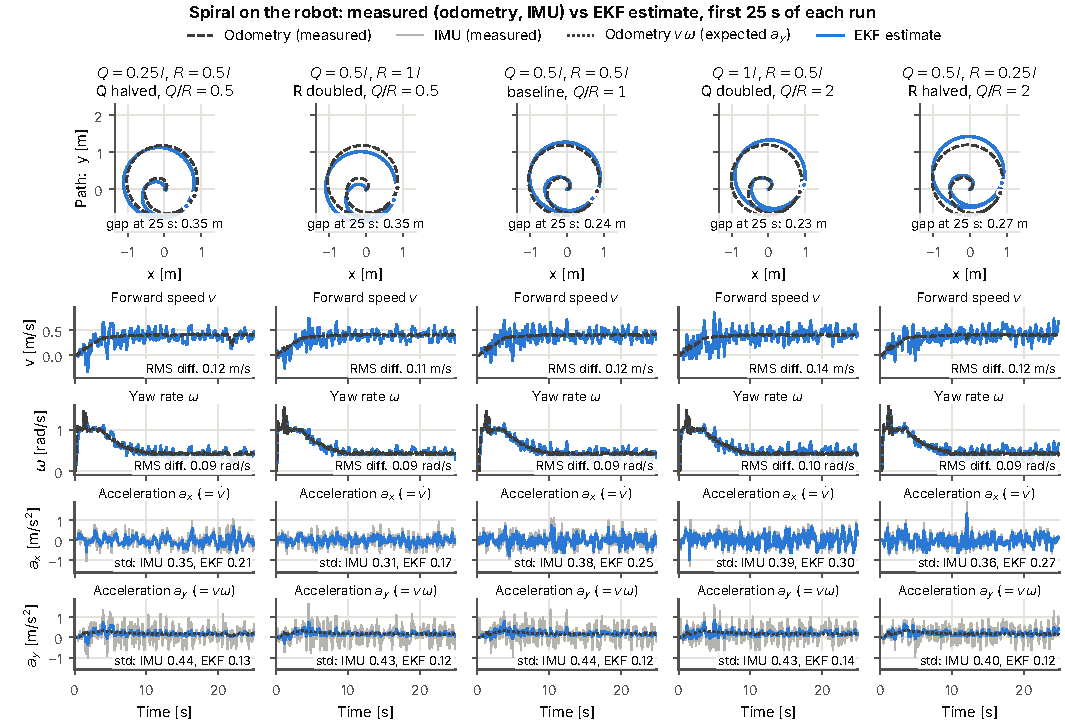
\includegraphics[width=\textwidth]{figures/fig_spiral.pdf}
  \caption{Spiral, one column per setting, sorted by $Q/R$. In every run $\hat v$ and $\hat\omega$ follow the odometry, but have
  noise that the odometry does not have. The noise is from the IMU through the $a_y$ row: raw $a_y$ has a standard deviation
  of 0.40--0.44\,m/s$^2$. The noise integrates into the path, which ends 0.23--0.35\,m from the odometry after 25\,s
  ($\approx$9\,m driven). The estimate gets noisier as $\mat{Q}$ grows: the standard deviation of $\hat{\dot v}$ rises from 0.17--0.21
  to 0.27--0.30\,m/s$^2$. Columns with the same $Q/R$ behave alike.}
  \label{fig:spiral}
\end{figure}

\begin{figure}[H]
  \centering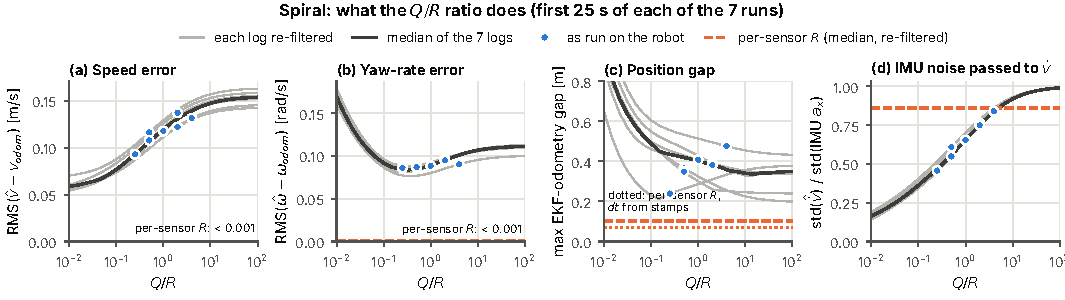
\includegraphics[width=\textwidth]{figures/fig_ratio.pdf}
  \caption{Effect of $Q/R$ on the spiral. Only the blue dots are robot runs. Curves are a simulation:
  the measurements logged in each run, passed again through the same EKF equations with $Q/R$ swept from
  0.01 to 100. Ratios tested in lab lie where the curves
  are mostly flat, which is why the columns of Fig.~\ref{fig:spiral} look similar. (a, d) Higher $Q/R$ passes
  more IMU noise. (b) A lower $Q/R$ smooths but lags, benefits of smoothing overcome by lag at about 0.2.
  (c) The lag during the spiral-out becomes a heading error, so the gap is largest at low $Q/R$.}
  \label{fig:ratio}
\end{figure}

\para{Point controller (Fig.~\ref{fig:point}).} Goal $(-1,-1)$\,m, EKF position is the controller's feedback, 1\,cm goal tolerance.
Final tuning parameters: $\mat{Q}=0.25\,\mat{I}$, $\mat{R}=1\,\mat{I}$.
This $Q/R=0.25$ is near the yaw-rate error minimum (Fig.~\ref{fig:ratio}b), passes less than half of the IMU noise (Fig.~\ref{fig:ratio}d) and gave the smallest maximum gap in our spiral runs (0.24\,m).
The EKF reports the goal has been reached after 21.2\,s, when the odometry put the robot at $(-0.98,-0.94)$\,m, 6\,cm from the EKF estimate.

\begin{figure}[H]
  \centering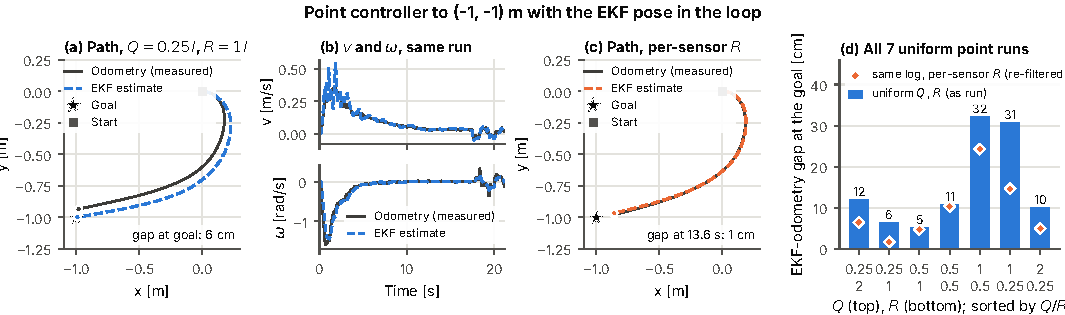
\includegraphics[width=\textwidth]{figures/fig_point.pdf}
  \caption{(a, b) Final uniform tuning. The largest differences are in the first 3\,s, when the robot turns $135^\circ$ at up to
  1.6\,rad/s; the heading error from this section becomes the offset along the rest of the path. (c) Per-sensor $\mat{R}$ on the robot (taken from Lab~1) sensor data:
  within $\sim$3\,cm of the odometry. From 13.6\,s (0.15\,m before the goal) the robot bumps into another robot, and the run was
  stopped; this is not shown. (d) Gap when the EKF declared the goal reached, single runs: 5--32\,cm.}
  \label{fig:point}
\end{figure}

%=====================================================================================================
\section{Discussion: how \texorpdfstring{$\mat{Q}$}{Q} and \texorpdfstring{$\mat{R}$}{R} affect the estimate}\label{sec:disc}

\para{Raising $Q/R$.} This tells the filter that the model is poor or the sensors are trustworthy. All
Kalman gains rise, so the estimate follows each new measurement quickly and sensor noise passes through: re-filtering the
seven logs, the speed error grows from 0.09\,m/s at $Q/R=0.2$ to 0.14\,m/s at $Q/R=5$, and the fraction of raw $a_x$ noise left in
$\hat{\dot v}$ from 0.44 to 0.86.
\textbf{Lowering $Q/R$.} This makes the filter trust the model (constant-$\omega$, constant-$\dot v$) more: the
estimate is smooth, but reacts slowly whenever the robot does something else (e.g., the ramp and the tightening spiral). When simulating $Q/R=0.01$ the yaw-rate
error doubles to 0.17\,rad/s and the path gap reaches $\sim$1\,m. For our data the best compromise is $Q/R\approx0.2$--0.5.

\para{Uniform $\mat{R}$ Assumption.}

Using a uniform $R$ appears to have a more significant effect than the $Q/R$ ratio.
One number cannot describe four sensors of very different quality.
Our Lab~1 logs (steady part of the run) give variances of about $2\times10^{-5}$\,(m/s)$^2$ for $v$
and $2\times10^{-4}$\,(rad/s)$^2$ for $\omega$ (odometry heading differenced), and 0.05 and 0.06\,(m/s$^2$)$^2$ for $a_x$ and $a_y$.
With $\mat{R}=r\,\mat{I}$ the centripetal row pulls $\hat v$ away from the odometry's reported measurement, which is over 1000 times less noisy.
We therefore also tried $\mat{R}=\mathrm{diag}(2\times10^{-5},\,2\times10^{-4},\,0.05,\,0.06)$ with $\mat{Q}=0.25\,\mat{I}$.
The gains on the odometry become 1.00 and the gain from $a_y$ to $v$ falls from 0.20 (uniform $\mat{R}$, $Q/R=1$) to 0.0001, so the IMU is used only for $\dot v$.
In lab, the estimate stayed within about 3\,cm of the odometry (Fig.~\ref{fig:point}c).
Re-filtering the seven spiral logs gives speed and yaw-rate errors below 0.001\,m/s and 0.001\,rad/s and a median path gap of 0.10\,m instead of 0.38\,m (Fig.~\ref{fig:ratio}).

\para{Unavoidable Error.} 

(1) The position is never measured, so an error in $\hat v$ or $\hat\omega$ stays in the path for the rest of the run, and a robot that is picked up and moved cannot find itself again.
Correcting for this requires a sensor that can directly measure position relative to the world (e.g., lidar and a map).
(2) The filter integrates with a fixed $dt=0.1$\,s, but consecutive samples are 0.03--0.26\,s apart.
Taking $dt$ from the stamps lowers the median gap left with the per-sensor $\mat{R}$ from 0.10 to 0.07\,m (Fig.~\ref{fig:ratio}c).

\end{document}
